% !TeX encoding = UTF-8
\documentclass{article}

\usepackage{CJKutf8}
\usepackage{enumitem}
\usepackage{multirow}
\usepackage{amsmath}
\usepackage{graphicx}
\usepackage{subcaption}
\usepackage{setspace}
\usepackage{wallpaper}
\usepackage{adjustbox}
\usepackage{afterpage}
\usepackage{lscape}
\usepackage{mathptmx}
\usepackage{titlesec}
\usepackage[hyphens]{url}
\usepackage[margin=2.8cm]{geometry}
\addtolength{\wpXoffset}{+9.26cm}
\addtolength{\wpYoffset}{-12.5cm}
\usepackage[backend=bibtex]{biblatex}

\bibliography{main}

\usepackage{booktabs}
\usepackage{siunitx} % Required for alignment
\sisetup{
  round-mode = places, % Rounds numbers
  round-precision = 2, % to 2 places
}
\usepackage{listings}
\usepackage{color}

\renewcommand\lstlistingname{Figure}
\renewcommand\lstlistlistingname{Figures}

\DeclareCaptionLabelFormat{tablel}{#1 #2}
\captionsetup[table]{labelsep=period}
\captionsetup[figure]{labelsep=period}

\lstset{
  language=XML,
  morekeywords={encoding,
  xs:schema,xs:element,xs:complexType,xs:sequence,xs:attribute}
  }
  % \setlist[description]{leftmargin=\parindent,labelindent=\parindent}

  % 以深度學習辨識中文文本蘊涵關係

  \title{Recognizing Chinese Textual Entailment by Deep Learning}
  \author{
    Wei-Ting Chen\\
    National Taiwan Ocean University\\
    \texttt{10757025@mail.ntou.edu.tw}\\
    \\
    Chuan-Jie Lin\\
    Nation Taiwan Ocean University\\
    \texttt{cjlin@mail.ntou.edu.tw}\\
    }

    \begin{document}
    \begin{CJK*}{UTF8}{bkai}

      \begin{titlepage}
  \centering
  {\Huge 國立臺灣海洋大學\par}
  \vspace{1cm}
  {\huge 資訊工程學系\par}
  \vspace{1cm}
  {\huge 碩士學位論文\par}
  \vspace{2cm}
  {\LARGE 指導教授:林川傑\ (Lin, Chuan-Jie) 博士\par}
  \vfill
  {\LARGE 以深度學習辨識中文文本蘊涵關係\par}
  {\LARGE Recognizing Chinese Textual Entailment by Deep Learning\par}
  \vfill
  {\LARGE 研究生:陳威廷\ \bigg(
    \begin{tabular}{c}
      Chen, Wei-Ting \\
      M00000000
    \end{tabular}
    \bigg) 撰}
    \vfill
    {\LARGE 中華民國\ 110 年\ 03 月}
  \end{titlepage}

  \newpage

  \begin{titlepage}
    \centering
  {\LARGE 以深度學習辨識中文文本蘊涵關係\par}
  \vfill
  {\LARGE Recognizing Chinese Textual Entailment by Deep Learning\par}
  \vfill
  {
    \LARGE
    \begin{minipage}{2in}
      研究生:陳威廷 \\
      指導教授:林川傑
    \end{minipage}
    \hfill
    \begin{minipage}{2.4in}
      Student: Chen, Wei-Ting \\
      Advisor: Lin, Chuan-Jie
    \end{minipage}
    \par
    }
    \vfill
    {\LARGE 國立臺灣海洋大學\par}
    {\LARGE 資訊工程學系\par}
    {\LARGE 碩士學位論文\par}
    \vfill
    {
      \LARGE
      A Thesis \\
      Submitted to Computer Science and Engineering \\
      Electrical Engineering and Computer Science \\
      National Taiwan Ocean University \\
      In Partial Fulfillment of the Requirements \\
      for the Degree of \\
      Master of Science \\
      in \\
      Computer Science and Engineering \\
      March, 2021 \\ \vspace{0.5cm}
      Keelung, Taiwan, Republic of China
      }
      \vfill
      {\LARGE 中華民國\ 110 年\ 03 月}
\end{titlepage}

\pagenumbering{gobble}

\newpage

\CenterWallPaper{0.1}{ntou.png}
\doublespacing
\tableofcontents
\singlespacing

\newpage

\listoffigures
\listoftables

\newpage

\pagenumbering{arabic}

\titleformat{\section}{\newpage\centering\normalfont\huge}{Chapter \thesection.}{1em}{}
\section{Introduction} \label{section:introduction}

\subsection{Motivation}
\paragraph{}
% NLI 任務在定義上並不複雜,給定一句 Premise 和一句 Hypothesis,並辨識這兩句話是否存在蘊含關係。一個文意蘊含任務的分類有很多種類型,最簡單的分法就是「有蘊含」與「沒有蘊含」,而「沒有蘊含」的部份可以進一步的分成「互斥」與「獨立」,「有蘊含」的部份也可以進一步的分成「正向蘊含」與「雙向蘊含」。去判別兩句話之間是否存在蘊含關係,這個任務的難度會因為涉及的語言現象而產生很高的複雜度
The definition of the textual entailment (also called natural language inference) task is not complex, given a premise sentence and a hypothesis sentence, and recognizing if the two sentences are entailment. The category of the textual entailment tasks has many types, the simplest one is to divide into ``entailment'' and ``not entailment''. Further, ``not entailment'' can be divided into ``contradiction'' and ``independence'', and ``entailment'' can be divided into ``forward entailment'' and ``bi-directional entailment''. The determination of the relation of the two sentences will become highly difficult according to the complexity of the linguistic phenomenon that the sentences involved.

\paragraph{}
% 模型是否能夠精準判別此蘊含關係,是衡量此模型的自然語言理解能力很重要的指標。在許多自然語言的應用中,例如:問答系統、文件摘要、資訊擷取與機器翻譯等,若是能提高模型的語言理解能力,將會是相當有幫助的事情。
Whether a model can accurately inference the relation of the sentences is quite important a indicator to measure the natural language understanding ability of the model. Increasing the NLU ability of the model will be helpful in many applications of the NLP, for example, question-answering system, summarization, information extraction, and machine translation.

\paragraph{}
% 近年來深度學習在 NLI 任務上取得了巨大的成功,但多數的成果都是僅限於大型英文資料集。本論文將會以繁體中文的 NLI 資料集 - RITE 為主要目標,將這份成功帶到這份相對小型的繁體中文資料集上面。
Deep learning has achieved huge success on the NLI tasks, but most of them on restricted to large-scale English datasets. This thesis will use the Traditional Chinese NLI datasets, RITE, as the main target, to try to bring success into these relatively small-scale datasets.

\subsection{Related Work}
\paragraph{}
In English NLI datasets, the Stanford Natural Language Inference (SNLI)\cite{snli:emnlp2015} is a well-known corpus of the NLI datasets, which is a collection of 570k human-written English sentence pairs. GLUE benchmark collected some datasets as their NLT task benchmark, including RTE, MNLI, QNLI, WNLI. The Recognizing Textual Entailment (RTE) datasets come from a series of annual textual entailment challenges. RTE1\cite{dagan2006pascal}, RTE2\cite{bar2006second}, and RTE3\cite{giampiccolo2007third} are provided from PASCAL\footnote{http://pascallin.ecs.soton.ac.uk/}, RTE4, RTE5\cite{bentivogli2009fifth}, RTE6, and RTE7 are provided from NIST\footnote{https://www.nist.gov/}. The Multi-Genre Natural Language Inference (MultiNLI, or MNLI)\cite{N18-1101} is a crowd-sourced collection of 433k sentence pairs collected from a wide range of genres. Question-answering NLI (QNLI)\cite{wang2019glue} dataset is an NLI dataset converting from the Stanford Question Answering Dataset v1.1 (SQuAD)\cite{rajpurkar2016squad}. The Winograd NLI dataset (WNLI) is also an augmented dataset, which is come from a reading comprehension task called The Winograd Schema Challenge\cite{levesque2011winograd}.

\paragraph{}
In Chinese NLI datasets, Chinese Natural Language Inference (CNLI)\footnote{https://github.com/blcunlp/CNLI} is a Simplified Chinese dataset from a sub task of The Seventeenth China National Conference on Computational Linguistics (CCL 2018) which has 90k sentence pairs. Original Chinese Natural Language Inference (OCNLI) is a NLI dataset with 50k sentence pairs, and it is a part of CLUE benchmark\footnote{https://www.cluebenchmarks.com/}. In NTCIR-9\cite{ntcir9rite1}, NTCIR-10\cite{ntcir10rite2}, and NTCIR-11\cite{ntcir11rite-val}, they proposed the RITE datasets, which have Japanese, Traditional Chinese, and Simplified Chinese task.
% Related NLI dataset, RTE\cite{dagan2006pascal}\cite{bar2006second}\cite{giampiccolo2007third}, SNLI, MNLI, QNLI\cite{wang2019glue}, CNLI, OCNLI, RITE.

% 與我們同實驗室的 Tu 等人在 RITE1 與 RITE2 的 BC Task 上取得了 71.05% 與 66.62% 的 F-scores,而在 MC Task 上則達到 53.27% 與 48.39% 的 F-scores. 這些成果都比 NTCIR-9 與 NTCIR-10 的參賽系統都來得好。之後的 Liu 等人則擴展了上個方法,將之應用在 RITE-VAL 上,其效能也同樣勝過 NTCIR-11 的參賽系統。
\paragraph{}
Zanzotto et al. (2006)\cite{zanzotto_moschitti_2006} conduct the experiments with the datasets of the RTE 2005 challenge by using cross-pair similarities. Wang et al. (2007) have achieved an accuracy of 66.9\% on the RTE-3 dataset by using sentence similarity based on dependency tree skeletons. Dinu et al. (2009)\cite{dinu_wang_2009} focused on the inference rules and try to find the improvement. Su et al.\cite{su_zheng_2011} achieved the best performance on NTCIR-9 RITE by using C4.5 decision tree base on the lexical and semantic features. Wang et al. (2013)\cite{wang-etal-2013-labeled} achieved the best performance on NTCIR-10 RITE2 (Simplified Chinese) by labeled alignment. Tu et al. (2015)\cite{tu_2015} using the rule-based classifier and combine with the SVM classifier, reached the F-scores of 71.05\% and 66.62\% to the BC task of RITE1 and RITE2, and the F-scores of 53.27\% and 48.39\% to the MC task, all of them are better than the best system of NTCIR-9 and NTCIR-10. Liu et al. (2016)\cite{liu_2016} expanded the methods and applied them on RITE-VAL, which has a better performance compared with the best system of NTCIR-11.

% BERT 2018, RoBERTa 2019, ALBERT 2019, SemBERT 2019, MTDNN 2019, XLNet 2019
% Vaswani 等人提出了 Attention 機制,並使用該機制創造了 Transformers 架構,在機器翻譯上取得了不錯的成績。Devlin 等人則將 Transformer 架構進一步擴展到多個 NLU 任務上面,取得了巨幅的成功。之後的 RoBERTa (Liu et al., 2019), ALBERT (Lan et al., 2020), SemBERT (Zhang et al., 2020), MTDNN (Liu et al., 2019), XLNET (Yang et al., 2020), T5 (Raffel et al., 2020), ERNIE (Zhang et al., 2020), DeBERTa (He et al., 2021)
\paragraph{}
Vaswani et al. (2017)\cite{vaswani2017attention} create the attention mechanism and create the architecture of transformers, achieved a great performance on machine translation task. Devlin et al. (2018)\cite{devlin2018bert} expanded the transformers onto many NLU tasks and achieved a huge success. RoBERTa (Liu et al., 2019)\cite{liu2019roberta} optimized the pretraining approach of BERT. ALBERT (Lan et al., 2020)\cite{lan2020albert} reduced the parameters of BERT and achieve a better performance than BERT. SemBERT (Zhang et al., 2020)\cite{zhang2020sembert} incorporate the contextual semantics to improve the results on reading comprehension task. Liu et al. (2019)\cite{liu2019mtdnn} proposed MT-DNN make the language representation more general to adapt to new tasks and domains. XLNET (Yang et al., 2020)\cite{yang2020xlnet} is a generalized autoregressive pretraining method that overcomes the limitations of BERT. T5 (Raffel et al., 2020)\cite{raffel2020t5} used a unified text-to-text transformer to explore the limits of transfer learning. ERNIE (Zhang et al., 2019)\cite{zhang2019ernie} take full advantage of lexical, syntactic, and knowledge information of the knowledge graphs to train an enhanced language representation model. DeBERTa (He et al., 2021)\cite{he2021deberta} uses the disentangled attention mechanism and the enhanced mask decoder to improve the efficiency of the model pretraining and the model performance. The success of these models is benefited from the transformers architecture.

\subsection{Thesis Architecture}
\paragraph{}
% 本論文的章節編排如下:我們首先會在第二章介紹與分析實驗所需使用到的資料集。在第三章會解說實驗會用到的方法與這些方法所需用到的資源。實驗結果與分析將會放在第四章。而第五章會總結本論文的研究成果與未來可以改進的方向。
The chapters of this thesis are organized as follows: We will introduce and analyze the datasets we used in chapter \ref{section:datasets}. In chapter \ref{section:approaches}, we will explain the methods and the resources that using in the methods. Then we introduce the pseudo training data in chapter \ref{section:pseudo} to improve our system. The results of the experiments will be discussed in chapter \ref{section:experiments}. Finally, we will conclude in chapter \ref{section:conclusion} and propose the direction of improvement.

\section{Datasets} \label{section:datasets}
\paragraph{}
% NLI 資料集是數組句對的集合,每組句對由一個「前提句」與一個「假設句」所組成,這兩句話會形成一個推論,用來表示兩句話之間的關係,這樣的任務被稱為 NLI / RTE。而本論文主要研究的對象 - RITE 資料集則是使用了雙向、單向、互斥與獨立四個關係。
An NLI dataset is a collection of sentence pairs, each sentence pairs, premise and hypothesis, has an inference, which indicates the relation of two sentences, this kind of task is known as natural language inference (NLI), also known as recognizing textual entailment (RTE). In this section, we will introduce the datasets that we use in our experiments.

\paragraph{}
% 常見的 NLI 資料集例如 SNLI, MNLI 與 CNLI 等,通常使用了蘊含、互斥與獨立三個標籤,我們稱之為 ECN Task。這些標籤的含意如下:
The relations of common NLI datasets, for example SNLI\cite{snli:emnlp2015}, MNLI\cite{N18-1101}, CNLI\footnote{https://github.com/blcunlp/CNLI}, and OCNLI\cite{ocnli}, usually represent in three types of labels: entailment, contradiction, and neural, we called these dataset as ECN task. The meaning of these labels are as following:

\subparagraph{entailment} means that the premise entails the hypothesis, and whether the hypothesis entails the premise does not matter.
\begin{table}[ht!]
  \centering
  \begin{tabular}{|c|l|}
    \hline
    Premise & The way we try to approach it is to identify every legal problem that a client has. \\ \hline
    Hypothesis & All of the client's legal problems are supposed to be identified. \\ \hline
  \end{tabular}
  \caption[An example of an entailment pair from MNLI]{An example of an entailment pair from MNLI. Both of the sentences are talking about identifying the legal problems of the client, so the inference of the sentence pair is ``entailment''.}
\end{table}

\subparagraph{contradiction} means that the premise and the hypothesis cannot be true at the same time.

\begin{table}[ht!]
  \centering
  \begin{tabular}{|c|l|}
    \hline
    Premise & There was food for all, and houses had been conjured hastily to shelter the people. \\ \hline
    Hypothesis & There was not enough food for all sadly. \\ \hline
  \end{tabular}
  \caption[An example of a contradiction pair from MNLI]{An example of a contradiction pair from MNLI. The premise says that the food is enough but the hypothesis says it is not, so the inference of the sentence pair is ``contradiction''.}
\end{table}

\subparagraph{neural} means that the premise does not have any relation mentioned above with the hypothesis.

\begin{table}[ht!]
  \centering
  \begin{tabular}{|c|l|}
    \hline
    Premise & Well i think that's about all my pet stories right now so. \\ \hline
    Hypothesis & My pets are up to many antics, and I'm happy I got to share these. \\ \hline
  \end{tabular}
  \caption[An example of a neutral pair from MNLI]{An example of a neutral pair from MNLI. The premise is talking about the story of the pet, but the hypothesis is talking about the antics of the pet, they are irrelevant to each other, so the inference of the sentence pair is ``neutral''.}
\end{table}

\paragraph{}
And in this thesis, our main target datasets - RITE, have four types of labels: B (bi-directional entailment), F (forward entailment), C (contradiction), and I (independence), we called these dataset as BFCI task.

\subparagraph{bi-directional entailment} means that the premise entails the hypothesis, and the hypothesis entails the premise.

\begin{table}[ht!]
  \centering
  \begin{tabular}{|c|l|}
    \hline
    Premise & 約瑟夫·傅立葉是十九世紀法國數學家及物理學家。 \\ \hline
    Hypothesis & 十九世紀法國的約瑟夫·傅立葉是數學家、物理學家。 \\ \hline
  \end{tabular}
  \caption[An example of a bi-directional entailment pair from RITE-VAL]{An example of a bi-directional entailment pair from RITE-VAL. The hypothesis is a paraphrase of the premise, they are talking about the same thing, so the inference of the sentence pair is ``bi-directional entailment''.}
\end{table}

\subparagraph{forward entailment} means that the premise entails the hypothesis, but the hypothesis does not entail the premise.

\begin{table}[ht!]
  \centering
  \begin{tabular}{|c|l|}
    \hline
    Premise & 約瑟夫·傅立葉是十九世紀法國數學家、物理學家。 \\ \hline
    Hypothesis & 約瑟夫·傅立葉是物理學家。 \\ \hline
  \end{tabular}
  \caption[An example of a forward entailment pair from RITE-VAL]{An example of a forward entailment pair from RITE-VAL. The premise says that Joseph Fourier is a person of 19 century, but the hypothesis does not mention the 19 century, so the premise can entail the hypothesis but the hypothesis can not entail the premise, this pair is marked as forward entailment.}
\end{table}

\subparagraph{contradiction} as same as the meaning in the ECN task.

\subparagraph{independence} as same as the meaning of neural in the ECN task.

\paragraph{}
In addition to the BFCI task and the BC task, both of them can be converted to BC task which is short for the binary classification task. The label of ``entailment'', ``bi-directional entailment'', and ``forward entailment'' will be marked as ``true'', and the label of ``contradiction'', ``neural'', and ``independence'' will be marked as ``false''.

\subsection{RITE}
\paragraph{}
RITE (Recognizing Inference in TExt) is the sub task in NTCIR conference, including Traditional Chinese, Simplified Chinese, and Japanese. In this research, we use the Traditional Chinese of RITE2 and RITE-VAL as our major evaluation datasets, which are come from NTCIR-10\cite{ntcir10rite2} and NTCIR-11\cite{ntcir11rite-val} these two conferences separately. They are collected from variety topics, such as domestic, history, politics, medicine and economy.

% 在 NTCIR-9 的時候同樣有舉辦 RITE 的 Task,其資料集為 RITE1,然而他的 dev set 與 test set 都被放入 RITE2 的 dev set 裡面,所以本研究只有使用 RITE2。
\paragraph{}
There is a RITE task in NTCIR-9 too, and the dataset it used is called RITE1\cite{ntcir9rite1}. However, the training set and test set of RITE1 had been merged into the training set of RITE2, so we only use RITE2 in this research.

\paragraph{}
% RITE-VAL 與 RITE2 的格式基本上相同,他們都有前提句 t1 與假設句 t2 以及他們的 id 與 label,而 RITE-VAL 則額外提供了「種類」的資訊,用來表示他們的句對其推論關係所涉及到的語言現象。
The formatting of RITE-VAL and RITE2 are the same, they both have the premise $t_1$, the hypothesis $t_2$, their pair id, and the label, while RITE-VAL provides the information of "category" to indicate the linguistic phenomenon of the relation of the sentence pair. RITE-VAL also includes the reversed labels in the training set. There are 28 linguistic phenomena are defined in RITE-VAL and listed in table \ref{tab:linguistic_phenomenon}. We only use this information to split RITE-VAL into 10 folds, and it is not a critical role in our experiments, so we didn't give a detailed description of the phenomenon.
% phenomenon - singular, phenomena - plural
\begin{table}[ht!]
  \centering
  \subfloat[The linguistic phenomenon related to entailment]{
    \begin{tabular}{|l|r|r|}
      \hline
      Category & Training & Test \\ \hline
      abbreviation & 6 & 25 \\ \hline
      apposition & 7 & 25 \\ \hline
      case\_alternation & 21 & 27 \\ \hline
      clause & 25 & 59 \\ \hline
      coreference & 11 & 24 \\ \hline
      hypernymy & 30 & 27 \\ \hline
      inference & 75 & 184 \\ \hline
      lexical\_entailment & 12 & 29 \\ \hline
      list & 20 & 37 \\ \hline
      meronymy & 4 & 23 \\ \hline
      modifier & 37 & 131 \\ \hline
      paraphrase & 47 & 49 \\ \hline
      quantity & 11 & 29 \\ \hline
      relative\_clause & 6 & 36 \\ \hline
      scrambling & 27 & 35 \\ \hline
      spatial & 18 & 42 \\ \hline
      synonymy:lex & 48 & 51 \\ \hline
      temporal & 11 & 40 \\ \hline
      transparent\_head & 13 & 26 \\ \hline
    \end{tabular}
  }
  \quad
  \subfloat[The linguistic phenomenon related to contradiction]{
    \begin{tabular}{|l|r|r|}
      \hline
      Category & Training & Test \\ \hline
      antonym & 20 & 35 \\ \hline
      exclusion:common\_sense & 8 & 34 \\ \hline
      exclusion:modality & 12 & 38 \\ \hline
      exclusion:modifier & 14 & 33 \\ \hline
      exclusion:predicate\_argument & 51 & 38 \\ \hline
      exclusion:quantity & 6 & 29 \\ \hline
      exclusion:spatial & 14 & 32 \\ \hline
      exclusion:temporal & 7 & 34 \\ \hline
      negation & 20 & 28 \\ \hline
    \end{tabular}
  }
  \caption{The linguistic phenomena distribution in RITE-VAL.}
  \label{tab:linguistic_phenomenon}
\end{table}

\paragraph{}
% RITE2 的 dev set 有 1321 組句對,test set 有 881 組句對,RITE-VAL 的 dev set 有 581 組句對,test set 有 1200 組句對。雖然 RITE2 資料量較多,但他們都是小規模的資料集。
RITE2 has 1,321 sentence pairs in the training set and 881 sentence pairs in the test set, while RITE-VAL has 581 sentence pairs in the training set and 1,200 sentence pairs in the test set. Though the data size of RITE2 has a little more, they are both small-scale datasets.

\begin{table}[ht!]
  \centering
  \begin{tabular}{|l|r|r|r|r|}
    \hline
    \multirow{2}{*}{Label} & \multicolumn{2}{c|}{RITE2} & \multicolumn{2}{c|}{RITE-VAL} \\
    \cline{2-5}
    & Training & Test & Training & Test \\ \hline
    B & 262 & 151 & 222 & 300 \\ \hline
    F & 544 & 328 & 148 & 300 \\ \hline
    C & 254 & 114 & 152 & 300 \\ \hline
    I & 261 & 288 & 59 & 300 \\ \hline
  \end{tabular}
  \caption{The label distribution of RITE2 and RITE-VAL.}
\end{table}

\paragraph{}
The table \ref{result:bfci_ntcir} and \ref{result:bc_ntcir} show the best results of RITE from NTCIR, both on the BFCI task and the BC task. The table \ref{result:bfci_liu_2016} and \ref{result:bc_liu_2016} show the best results of RITE of Liu et al., 2016.
% The best system of RITE2 is from Shih et al., 2013\cite{Shih2013IASLRS}.

\lstset{
  extendedchars=false,
  basicstyle=\ttfamily,
  keywordstyle=\color{blue},
  stringstyle=\color{purple},
  frame=lines,
  breaklines=true,
  showstringspaces=false,
  escapechar=\#,
}
% RITE2
\begin{figure}[ht!]
  \centering
  \caption{The examples of RITE2 and RITE-VAL}
  \begin{subfigure}{1\linewidth}
    \caption{Example of RITE2. The premise means "long-term use of steroids can cause emotional instability, hallucinations, and delusions" and the hypothesis means "steroids may cause hallucinations and delusions". The premise can inference the hypothesis but the hypothesis cannot inference the premise because it lack of the description of "emotional instability", so this example will be marked as "forward entailment".}
    \begin{minipage}{\linewidth}
    \begin{lstlisting}[language=XML]
    <pair id="430" label="F">
      <t1>#長期使用類固醇會導致情緒不穩,幻覺和妄想症#</t1>
      <t2>#類固醇可能造成幻覺妄想症#</t2>
    </pair>
    \end{lstlisting}
    \end{minipage}
    % 因為前提句
  \end{subfigure}

  % RITE-VAL
  \begin{subfigure}{1\linewidth}
    \caption{Example of the RITE-VAL training set, the column "category" show the relation of two sentences while the "吉力馬札羅火山" is an abbreviation of "吉力馬札羅山火山", so this pair is marked as "bi-directional".}
    \begin{minipage}{\linewidth}
    \begin{lstlisting}[language=XML]
    <pair id="1" label="B" revlabel="B" category="abbreviation">
      <t1>歷史上沒有吉力馬札羅山火山噴發的記錄。</t1>
      <t2>歷史上沒有吉力馬札羅火山噴發的記錄。</t2>
    </pair>
    \end{lstlisting}
    \end{minipage}
  \end{subfigure}
\end{figure}


\begin{table}[ht!]
  \centering
  \begin{tabular}{|l|r|r|r|r|r|}
  \hline
   & \multicolumn{1}{c|}{B-F1} & \multicolumn{1}{c|}{F-F1} & \multicolumn{1}{c|}{C-F1} & \multicolumn{1}{c|}{I-F1} & \multicolumn{1}{c|}{Macro F1} \\ \hline
  RITE-VAL & 0.4721 & 0.5206 & 0.4776 & 0.1511 & 0.4054 \\ \hline
  RITE-VAL-TEST & 0.6607 & 0.8296 & 0.4816 & 0.6185 & 0.6476 \\ \hline
  RITE2-TEST & 0.5235 & 0.6463 & 0.2990 & 0.3841 & 0.4632 \\ \hline
  \end{tabular}
  \caption{The best results of BFCI task from NTCIR-10 and NTCIR-11.}
  \label{result:bfci_ntcir}
\end{table}

\begin{table}[ht!]
  \centering
  \begin{tabular}{|l|r|r|r|}
  \hline
   & \multicolumn{1}{c|}{Y-F1} & \multicolumn{1}{c|}{N-F1} & \multicolumn{1}{c|}{Macro F1} \\ \hline
  RITE-VAL & 0.5672 & 0.5577 & 0.5624 \\ \hline
  RITE-VAL-TEST & 0.7894 & 0.6997 & 0.7446 \\ \hline
  RITE2-TEST & 0.7166 & 0.6263 & 0.6714 \\ \hline
  \end{tabular}
  \caption{The best results of BC task from NTCIR-10 and NTCIR-11.}
  \label{result:bc_ntcir}
\end{table}

\begin{table}[ht!]
  \centering
  \begin{tabular}{|l|r|r|r|r|r|}
  \hline
   & \multicolumn{1}{c|}{B-F1} & \multicolumn{1}{c|}{F-F1} & \multicolumn{1}{c|}{C-F1} & \multicolumn{1}{c|}{I-F1} & \multicolumn{1}{c|}{Macro F1} \\ \hline
  RITE-VAL & 0.6569 & 0.5438 & 0.5692 & 0.2209 & 0.4977 \\ \hline
  RITE-VAL-TEST & 0.5220 & 0.5592 & 0.5010 & 0.3623 & 0.4861 \\ \hline
  RITE2-TEST & 0.4720 & 0.6422 & 0.4052 & 0.4703 & 0.4974 \\ \hline
  \end{tabular}
  \caption{The best results of BFCI task from Liu et al., 2016.}
  \label{result:bfci_liu_2016}
\end{table}

\begin{table}[ht!]
  \centering
  \begin{tabular}{|l|r|r|r|}
  \hline
   & \multicolumn{1}{c|}{Y-F1} & \multicolumn{1}{c|}{N-F1} & \multicolumn{1}{c|}{Macro F1} \\ \hline
  RITE-VAL & 0.7425 & 0.5648 & 0.6536 \\ \hline
  RITE-VAL-TEST & 0.6766 & 0.5877 & 0.6321 \\ \hline
  RITE2-TEST & 0.7224 & 0.5992 & 0.6608 \\ \hline
  \end{tabular}
  \caption{The best results of BC task from Liu et al., 2016.}
  \label{result:bc_liu_2016}
\end{table}

\subsection{MNLI}
\paragraph{}
% MNLI 是一個透過 Crowd-sourced 建立的資料集,他蒐集了來自多種文體的句子,包含口說與書寫的文字。
MNLI (Multi-Genre Natural Language Inference, MultiNLI), as a dataset of GLUE benchmark, is a crowd-sourced large-scale dataset that collected sentences from a wide range of genres, both in spoken and written text. It has 392,702 sentence pairs in the training set and 10,000 in the dev set. Only the training set and dev set are public\footnote{https://cims.nyu.edu/~sbowman/multinli/}. The best system of MNLI is Raffel et al., 2020\cite{raffel2020t5}, which reached an accuracy of 92.0\%.

\begin{table}[ht!]
  \centering
  \begin{tabular}{|c|r|r|r|}
  \hline
  \multicolumn{1}{|l|}{} & \multicolumn{1}{c|}{Entailment} & \multicolumn{1}{c|}{Contradiction} & \multicolumn{1}{c|}{Neutral} \\ \hline
  MNLI-Train & 130,899 & 130,903 & 130,900 \\ \hline
  MNLI-Dev & 3,479 & 3,213 & 3,123 \\ \hline
  \end{tabular}
  \caption{The label distribution of MNLI.}
\end{table}

\begin{figure}
\caption[An example of MNLI]{An example of MNLI. There are five labels listed that from different annotators, and a gold label indicates which label annotated the most.}
\begin{minipage}{\linewidth}
\begin{lstlisting}[language=Python]
{
  "annotator_labels": [
      "neutral",
      "entailment",
      "neutral",
      "neutral",
      "neutral"
  ],
  "genre": "slate",
  "gold_label": "neutral",
  "pairID": "63735n",
  "promptID": "63735",
  "sentence1": "The new rights are nice enough",
  "sentence1_binary_parse": "( ( The ( new rights ) ) ( are ( nice enough ) ) )",
  "sentence1_parse": "(ROOT (S (NP (DT The) (JJ new) (NNS rights)) (VP (VBP are) (ADJP (JJ nice) (RB enough)))))",
  "sentence2": "Everyone really likes the newest benefits ",
  "sentence2_binary_parse": "( Everyone ( really ( likes ( the ( newest benefits ) ) ) ) )",
  "sentence2_parse": "(ROOT (S (NP (NN Everyone)) (VP (ADVP (RB really)) (VBZ likes) (NP (DT the) (JJS newest) (NNS benefits)))))"
}
\end{lstlisting}
\end{minipage}
\end{figure}

\subsection{CNLI}
\paragraph{}
CNLI (Chinese Natural Language Inference) is a Simplified Chinese dataset from a sub task of The Seventeenth China National Conference on Computational Linguistics (CCL 2018)\footnote{http://www.cips-cl.org/static/CCL2018/index.html}. It has 90,000 sentence pairs in the training set, 10,000 in the dev set and 10,000 in the test set which are all public available on GitHub\footnote{https://github.com/blcunlp/CNLI}. To understand the impact of Traditional Chinese characters and Simplified Chinese characters, we make a Traditional Chinese version called CNLI-TW.

\paragraph{}
From the official evaluation results\footnote{https://git.io/JIlih}, the best system achieve an accuracy of 82.38\%, and the second best system achieve an accuracy of 78.28\%.

\begin{table}[ht!]
  \centering
  \begin{tabular}{|c|r|r|r|}
  \hline
             & Entailment & Contradiction & Neutral \\ \hline
  CNLI-Train & 2,9738     & 2,8937        & 3,1325  \\ \hline
  CNLI-Dev   & 3,485      & 3,417         & 3,098   \\ \hline
  CNLI-Test  & 3,475      & 3,343         & 3,182   \\ \hline
  \end{tabular}
  \caption{The label distribution of CNLI.}

\end{table}
\begin{figure}
\caption{An example of CNLI}
\begin{CJK*}{UTF8}{gbsn}
\begin{lstlisting}[language=Python, escapechar=\#]
{
  "pid": "AE5175",
  "t1": "#\color{purple}穿红衬衫的男人和拿着白色袋子的女人正在交谈。#",
  "t2": "#\color{purple}两个人在交谈#",
  "label": "entailment"
}
\end{lstlisting}
\end{CJK*}
\end{figure}

\subsection{OCNLI}
\paragraph{}
OCNLI (Original Chinese Natural Language Inference) is also a large-scale Simplified Chinese NLI dataset that does not rely on the automatic translation or non-expert annotation. The sentences are collected from government documents, news, literature, TV show transcripts, and telephone conversation transcripts. It has 50,486 sentence pairs in the training set, 3,000 in the dev set, and 3,000 in the test set. Only the training set and the dev set are fully labeled and public available\footnote{https://github.com/CLUEbenchmark/OCNLI}, the test set only contained sentence pairs. Same as CNLI, we also make a Traditional Chinese version called OCNLI-TW.

\paragraph{}
The best system of OCNLI from the verified official leaderboard\footnote{https://www.cluebenchmarks.com/nli.html} is RoBERTa which achieved an accuracy of 77.30\%, and the second-best system is BERT, which reached an accuracy of 71.25\%.

\begin{table}[ht!]
  \centering
  \begin{tabular}{|c|r|r|r|}
  \hline
              & Entailment & Contradiction & Neutral \\ \hline
  OCNLI-Train & 16,779     & 16,476        & 17,182  \\ \hline
  OCNLI-Dev   & 947        & 900           & 1,103   \\ \hline
  \end{tabular}
  \caption{The label distribution of OCNLI.}
\end{table}

\begin{figure}
\caption{An example of OCNLI}
\begin{minipage}{\linewidth}
\begin{CJK*}{UTF8}{gbsn}
\lstset{emph={null},emphstyle={\color{cyan}}}
\begin{lstlisting}[language=Python, escapechar=\#]
{
  "level": "medium",
  "sentence1": "#\color{purple}经济社会发展既有量的扩大,又有质的提升,为今后奠定了基础#",
  "sentence2": "#\color{purple}经济社会始终在向好的方向发展#",
  "label": "neutral",
  "label0": null,
  "label1": null,
  "label2": null,
  "label3": null,
  "label4": null,
  "genre": "gov",
  "prem_id": "gov_96",
  "id": 50434
}
\end{lstlisting}
\end{CJK*}
\end{minipage}
\end{figure}

\section{Approaches} \label{section:approaches}
\subsection{Experiment Process}
\paragraph{}
% 我們將這部份分成特徵與分類器兩個部份來討論。在特徵的部份,我們重新製作了 Liu 等人提出的機器學習特徵,並提出了新的 CSA 方法製作新的特徵,同時也與一些常見的 NNLM 方法做比較。在分類器的部份,除了 Liu 等人使用的 SVM 分類器以外,也包含了單純的神經網路和 RNN 並結合 Attention 的機制,最後使用近年來在 NLP 領域相當受歡迎的 Transformer 模型 - BERT 做為分類器。
We will divide this part into the features and the classifiers to discuss. In the features, we remade the machine learning features mentioned in Liu et al., and proposed a new method called ``cosine similarity alignment''. Meanwhile, we compared these methods with some common language models. In the classifiers, in addition to the SVM classifier mentioned in Liu et al., we also used the simple neural network and the RNN model with attention mechanism. Finally, we will use a transformer model, BERT, which is popular in the NLP domain in recent years.

% 為了使用 Deep Learning 解決 NLI 問題並且與傳統機器學習方法做比較,我們首先重製了先前 Liu 等人使用的 ML 特徵與 SVM 的實驗,然後測試將 SVM 分類器改成簡單的 DNN 的效能如何。接下來,我們提出了 CSA 的方法,並將其放入深度學習的模型裡面。最後嘗試透過最近在 NLP 領域相當受歡迎的 BERT Transformer 模型來提升整體效能。
% \paragraph{}
% To solve the NLI problem by deep learning and compare the performance to the traditional machine learning methods, we first reproduce the machine learning feature extraction and the SVM experiment of Liu et al., then we test the performance of replacing the SVM classifier with a simple DNN classifier. And we propose a new method called ``Cosine Similarity Alignment'' that generate alignment features using cosine similarity of word vectors and feed it into RNN-attention neural network. Finally, we try to use the BERT transformer model which becomes popular in the NLP domain in recent years.

% 在重製傳統機器學習的部分,我們首先製作了在 Liu 等人 (2016) 提到的 Machine Learning Features,不過當時主要針對中文資料集來產生特徵,且使用的部分資源像是中文 WordNet 等已過於老舊,難以適用於現今的資料集,所以我們稍微修改了一部份的特徵產生方式,並同時設計了針對英文資料集的相同特徵。其中有部分特徵需要用到 Word Vectors 來產生,所以我們也使用了不同的 NNLM 來測試效果如何。
% \paragraph{}
% To reproduce the experiment of traditional machine learning, we first reproduce the features mentioned in Liu et al. (2016). But these features can only be applied to the Traditional Chinese datasets, and some resources like Traditional Chinese WordNet are too old to fit with the datasets nowadays. So we modified a little part of feature extraction and make the method compatible with the English datasets. Some of the features need to use the word vectors, so we use different language models to test the performance.

% 在 BERT 的實驗中,我們主要使用官方釋出的 bert-base-chinese 與 bert-multilingual-cased 兩個模型來進行實驗,並透過不同的資料集進行預訓練,最後再用 RITE 做 fine-tune。
% \paragraph{}
% In the experiment of BERT, we use the official released models and pre-training with different datasets then fine-tuning with the RITE datasets. At last, we try to merge the machine learning features and the cosine similarity alignment features into the BERT model.

\subsection{Machine Learning Features} \label{Features}
\paragraph{}
In this section, we will describe the features mentioned in Liu et al.\cite{liu_2016} and reproduce it. These features are used for machine learning originally, so we called these features as ``\textbf{ML Features}''.

\subsubsection{N-grams Features}
% Character N-gram Overlap & Word N-gram Overlap.
% Use CKIP-Tagger to do word segmentation.
\paragraph{}
% 讓 ngrams_1 and ngrams_2 為 t1 和 t2 所有的 n-grams,在只考慮內容詞的情況下計算 n-gram 一致的比例,同時也計算字與詞的版本
Let $ngrams_1$ and $ngrams_2$ be all n-grams of $t_1$ and $t_2$, calculate the proportion of n-grams overlap that are consistent with only content words, both the version of the words and the characters are calculated.

\begin{equation}
  overlap_1(ngrams_1,ngrams_2)=\frac{|ngrams_1\cap ngrams_2|}{|ngrams_1|}
\end{equation}

\begin{equation}
  overlap_2(ngrams_1,ngrams_2)=\frac{|ngrams_1\cap ngrams_2|}{|ngrams_2|}
\end{equation}

\paragraph{}
The features of n-grams overlap are listed below:

\setlist{noitemsep, topsep=5pt, parsep=0pt, partopsep=0pt, leftmargin=1.3cm, labelindent=1.2cm, labelwidth=\wd1, itemindent=*, labelsep=\dimexpr0.2cm-\wd1}

\begin{enumerate}
    \item[ 1.] n-grams overlap of characters $(t_1)$
    \item[ 2.] n-grams overlap of characters $(t_2)$
    \item[ 3.] n-grams overlap of words $(t_1)$
    \item[ 4.] n-grams overlap of words $(t_2)$
\end{enumerate}

\subsubsection{Grammer Features}
\paragraph{}
To generate grammar features, we use Stanza\cite{qi2020stanza} as the interface to Stanford Parser to parse the dependency of the sentences. Each dependency is composed of one relation and two arguments: the head and the modifier. These features are defined in Liu et al. (2016) and listed below:

\begin{enumerate}
    \item[ 5.] the proportion of the same relations $(t_1)$
    \item[ 6.] the proportion of the same relations $(t_2)$
    \item[ 7.] the proportion of the different relations $(t_1)$
    \item[ 8.] the proportion of the different relations $(t_2)$
    \item[ 9.] the proportion of the a same relation and a same argument but the other argument is different $(t_1)$
    \item[10.] the proportion of the a same relation and a same argument but the other argument is different $(t_2)$
    \item[11.] the proportion of the same arguments but different relation $(t_1)$
    \item[12.] the proportion of the same arguments but different relation $(t_2)$
    \item[13.] the proportion of the lack of the head $(t_1)$
    \item[14.] the proportion of the lack of the head $(t_2)$
    \item[15.] the proportion of the lack of the relation $(t_1)$
    \item[16.] the proportion of the lack of the relation $(t_2)$
\end{enumerate}

\subsubsection{Semantic Features}
\paragraph{}
Using NLTK\cite{nltk} with WordNet\cite{wordnet} to calculate WUP similarity\cite{wu-palmer-1994-verb}.

\begin{equation}
  wup(s_1,s_2)=\frac{2\times depth(lcs)}{depth(s_1)+depth(s_2)}
\end{equation}

\paragraph{}
% 我們可以使用 NLTK 來找到 LCS,並透過節點的深度計算出兩個 synsets 的相似度。因為每個內容詞可能有不只一個 synsets,所以我們定義兩個內容詞 c1 和 c2 的 wup 相似度如下
We can find the LCS (least common subsumer) with NLTK and calculate the depth of synsets to get WUP similarity. Because each content word may has more than one synset, we defined WUP similarity of content words $c_1$ and $c_2$ as following.

\begin{equation}
  sim(c_1,c_2)=\max\limits_{\substack{s_1\in synsets(c_1) \\ s_2\in synsets(c_2)}} wup(s_1,s_2)
\end{equation}

\paragraph{}
Harbin Institute of Technology Information Retrieval Lab\footnote{http://ir.hit.edu.cn/} Chinese Synonym Forest (or Tongyici Cilin) [Extended] lv5 Similarity

\begin{equation}
  lv5(C_1,C_2)=\frac{1}{|C_1|}\sum\limits_{c_1\in C_1}\max\limits_{c_2\in C_2} sim(c_1,c_2)
\end{equation}

\paragraph{}
% 因為中文的部份缺少完善的 WordNet 資源,而英文的部份則是缺少同義詞詞林的資源,所以這部份會透過 Cosine Similarity 來取代。
Because lack of a proper WordNet resource in Chinese and synonym forest in English, it is unable to calculate WUP similarity in Chinese and lv5 similarity in English. They will be replaced with the cosine similarity.

\begin{equation}
  similarity=\frac{A\cdot B}{||A||\ ||B||}=\frac{\sum\limits^{n}_{i=1}A_iB_i}{\sqrt{\sum\limits^{n}_{i=1}A^2_i}\sqrt{\sum\limits^{n}_{i=1}B^2_i}}
\end{equation}

\paragraph{}
The semantic features in English is listed below:

\begin{enumerate}
  \item[17.] average of cosine similarity $(t_1)$
  \item[18.] average of cosine similarity $(t_2)$
  \item[19.] average of WUP similarity $(t_1)$
  \item[20.] average of WUP similarity $(t_2)$
\end{enumerate}

\paragraph{}
The semantic features in Chinese is listed below:

\begin{enumerate}
  \item[17.] average of cosine similarity $(t_1)$
  \item[18.] average of cosine similarity $(t_2)$
  \item[19.] average of lv5 similarity $(t_1)$
  \item[20.] average of lv5 similarity $(t_2)$
\end{enumerate}

\subsection{Language Model}
\paragraph{}
The language models

\subsubsection{Self-trained Word Embedding}
\paragraph{}
Description of self-trained word embedding.

\subsubsection{fastText}
\paragraph{}
fastText\cite{bojanowski2016enriching} is a library for efficient text classification and representation learning created by Facebook's AI Research (FAIR) lab. This library allows us to create word embedding with unsupervised learning algorithms, like skip-gram and continuous bag-of-word (CBOW). With this library, we train a word representation from Traditional Chinese Wikipedia, both in the version of skip-gram and CBOW, the embedding size is 250.

\subsubsection{Google NNLM}
\paragraph{}
Google NNLM is provided by TensorFlow Hub\footnote{https://www.tensorflow.org/hub} which has many different language models that already be trained by a large corpus. We use the Chinese version of NNLM that trained on Simplified Chinese Google News 100B corpus and publish by Google\footnote{https://tfhub.dev/google/tf2-preview/nnlm-zh-dim128/1}. In order to fit the Traditional Chinese dataset, we convert the dictionary of the Google NNLM from Simplified Chinese into Traditional Chinese.
% BERT Language Model

\subsection{Cosine Similarity Alignment}
\paragraph{}
We propose a new method to do alignment by calculating the cosine similarity between words of two sentences and set a ``similarity threshold'' to define if the two words will be aligned. The similarity threshold is variable and we will observe the impact of the change of the value of the similarity threshold.

\paragraph{}
% 首先先計算兩句話的每個詞之間的 Cosine Similarity 建立一個 Similarity Table,然後從表中挑出相似數值最高的兩個詞,將 premise 的詞放入 list1 並將 hypothesis 的詞放入 list2,然後將這兩個詞從表中刪去,再繼續往下挑相似數值最高的兩個詞,直到該相似數值小於 Similarity Threshold 為止。接下來把 premise 剩下的詞一個一個放入 list1,每放一個詞到 list1 裡面,就在 list2 裡面放一個零,hypothesis 剩下的詞也是一樣的操作。最後將 list2 的值減去 list1 獲得最後的 CSA Features。
First, we calculated the cosine similarity of each word of two sentences to build a similarity table, then picked up the word pair with the highest value of similarity, and put the word vector of the word from the premise sentence into $list_1$ and put the one from the hypothesis sentence into $list_2$ and remove the two words from the similarity table. Repeat this step until the highest value of the similarity is lower than the similarity threshold. Next, we put the word vectors of the left words of the premise sentence into $list_1$ one by one, every time we put a word vector into $list_1$, put a zero vector into $list_2$, and do the same operation to the left words of the hypothesis sentence, so the two lists will remain the same size. After all, we use $list_2$ to minus $list_1$ to obtain the final ``CSA Features''.

\begin{figure}[!ht]
  \centering
  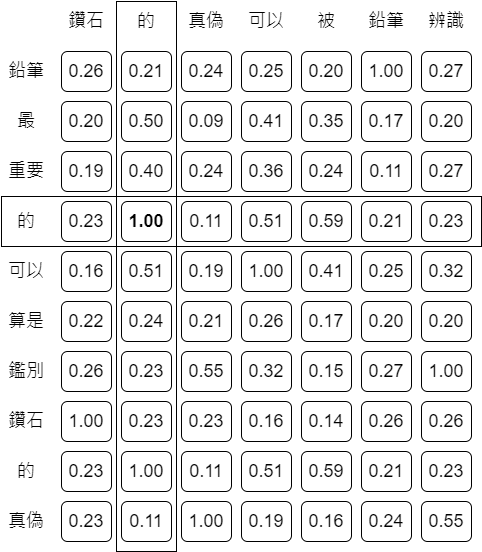
\includegraphics[width=175px]{CSA.png}
  % 此圖顯示兩句話裡每個字之間的 Cosine Similarity,每個字將會根據這個 Cosine Similarity Table 進行 Alignment
  \caption[Cosine Similarity Alignment]{This figure shows the calculation of cosine similarity between words of sentence pair, the words will be aligned by this cosine similarity table.}
  \label{fig:csa}
\end{figure}

\subsection{Classifier}

\subsubsection{Neural Network}
\paragraph{}
% 神經網路的蓬勃發展使機器學習在各領域上都獲得了不小幅度的進展,
% Dense Neural Network, Recursive Neural Network (LSTM, GRU), Attention Mechanism, Transformers
% Simple DNN 模型是只使用了一層 Dense Layer 的模型,透過 Tensorflow 套件建立而成。這個模型架構設計很單純,只用來接收 ML Features。
A simple DNN model is a model only using a dense layer, building by Tensorflow API. This model architecture is pretty simple, only use to receive machine learning features.

\subsubsection{RNN-Attention Model}
\paragraph{}
% RNN-Attention 模型是數種由不同數量與順序的 RNN Layers 與 Attention Layers 組合而成的模型
The RNN-Attention Model (RA Model) is a combination of several different numbers and orders of RNN layers and attention layers.

The attention mechanism is described in Vaswani et al. (2017)

\subsubsection{BERT}
\paragraph{}
The structure of transformer\cite{vaswani2017attention} has been described in Vaswani et al., 2017, they use multi-head attention to build the encoder-decoder model, which uses to solve the machine translation tasks. On the other hand, BERT\cite{devlin2018bert} (Devlin et al., 2019) also used the transformer architecture to achieve excellent performance on several natural language processing tasks, including MNLI, QNLI, and RTE which are contained in GLUE benchmark. The source code of BERT are available on GitHub\footnote{https://github.com/google-research/bert} and it can be easily called using HuggingFace Transformers API\cite{wolf-etal-2020-transformers}.

\paragraph{}
There are many different models from the official GitHub repository, like the \texttt{bert-base-cased} model is pre-trained by cased English corpus and the \texttt{bert-base-chinese} model is pre-trained by both Traditional Chinese and Simplified Chinese corpus. Besides these language-specific models, the most important model is the cross-lingual model like the \texttt{bert-base-multilingual-cased} model, which allows us to train and fine-tune with different languages in one model easily.

\section{Pseudo Training Data} \label{section:pseudo}
% 我們嘗試使用大量的虛擬資料來改進模型的效能,虛擬資料的產生方式則有規則式改寫與 GPT2 模型生成兩種。這兩種方法會對四個標籤都產生等量的資料,並根據 MNLI 的資料量,各產生 400k 組句對。在接下來的章節會介紹產生虛擬資料的細節。
\paragraph{}
We try to use large-scale pseudo dataset to improve the performance of the model, and the generating methods of the simulation data are rule-based rewriting and GPT2 model generation. Both of the methods will generate an equal amount of data for the four labels. According to the data size of the MNLI dataset, each of the methods will generate 400k sentence pairs. We will introduce the details of the simulation data generation in the following sections.

\subsection{Rule-Based}
% 在規則式的部份,我們首先使用替換法的方式來產生句對,替換的對象包含同義詞與反義詞。我們從 Corpus 中隨機挑選出一個由二到三個短句所構成的句子,並從句中尋找一個存在於同義詞辭典或反義詞辭典的詞來進行替換。同義詞辭典來自於同義詞詞林,而反義詞辭典則來自於中英 WordNet 的對應。因為可替換的詞可能不只一個,所以會優先使用字數相近的詞。接下來,我們嘗試在句中隨機加入否定詞。我們先計算了整個 Corpus 裡面否定詞詞性的 N-Gram 機率,再從隨機挑選的句子中尋找詞性 N-Gram 機率較高的位置插入否定詞。上述的做法都只會替換或插入一個詞。以同義詞替換而產生的句對被標記為 B,以反義詞替換而產生的句對被標記為 C,以隨機插入否定詞而產生的句對被標記為 C。
% TODO: 是否對於反義詞字典更詳細的介紹
\paragraph{}
In the rule-based method, we first use the substitution method to generate sentence pairs, and the targets of substitution include synonyms and antonyms. We randomly select a long sentence consisting of 2 to 3 short sentences from the corpus and search for a word from the existing sentences in the antonym or synonym dictionary to replace it. The synonym dictionary comes from HIT, and the antonym dictionary comes from the mapping of English WordNet and Chinese WordNet. Because there will be more than one word that can be replaced in a sentence, a similar number of characters will be used. Next, we try to add negative words into sentences randomly. We first calculate the n-gram probability of the sentences including negative words and insert a negative word into the position with the highest probability. The methods above will only replace or insert one word, the augmented sentence will be seen as the hypothesis and combined with the original sentence as new sentence pair. The sentence pairs generated by synonym substitution will be marked as ``bi-directional''. The sentence pairs generated by antonym substitution will be marked as ``contradiction''. The sentence pairs generated by negative word insertion will be marked as ``contradiction''.

% 為了更進一步擴展我們的資料集,我們將產生出來的句子以逗號為邊界,將句子分割成數個短句,並將這些短句與原本的句子重新組成新的句對。若是該短句沒有被改造過,則新的句對被標記為 F;若是該短句被改造過且原本被標記為 C,則新的句對同樣被標記為 C;若是該短句被改造過且原本被標記為 B,則新的句對會被標記為 F。
\paragraph{}
To further expand our dataset, we split the sentence into several short sentences according to the comma and combined each of these short sentences with the original sentences as new sentence pairs. If the new sentence has not been modified, the new sentence pair will be marked as ``forward entailment''. If the new sentence has been modified and originally marked as ``contradiction'', the new sentence pair will also be marked as ``contradiction''. If the new sentence has been modified and originally marked as ``bi-directional'', the new sentence will be marked as ``forward entailment''.

% 最後,我們使用兩種單純的方法來產生 I 的資料。第一種是從 Corpus 裡面隨機挑選兩句組成一個句對;第二種是從 Corpus 裡面挑選一個長句,並將其斷成前後兩句,由這兩句話組成一個句對。
\paragraph{}
Finally, we use two simple ways to generate ``independence'' sentence pairs. The first is to randomly pick two sentences from corpus as a sentence pair, the second is to randomly pick a long sentence from corpus, and split it into two sentence as new sentence pair.

% Synonmy
% 失控所致或營造而成,差異極大
% 失控所致或營造而成,反差極大
% Split 1
% 失控所致或營造而成,差異極大
% 失控所致或營造而成
% Split 2
% 失控所致或營造而成,差異極大
% 反差極大

% Antonym
% 即日起上市,可預約宅配
% 即日起上市,不許預約宅配
% Split 1
% 即日起上市,可預約宅配
% 即日起上市
% Split 2
% 即日起上市,可預約宅配
% 不許預約宅配

% Negative
% 相較之下,台灣藝術家以公共藝術文化輸出的案例卻未聽聞
% 相較之下,台灣藝術家以非公共藝術文化輸出的案例卻未聽聞
% Split 1
% 相較之下,台灣藝術家以公共藝術文化輸出的案例卻未聽聞
% 相較之下
% Split 2
% 相較之下,台灣藝術家以公共藝術文化輸出的案例卻未聽聞
% 台灣藝術家以非公共藝術文化輸出的案例卻未聽聞

\begin{table}[ht!]
  \centering
  \begin{tabular}{|l|l|c|}
    \hline
    \multicolumn{1}{|c|}{Method} & \multicolumn{1}{c|}{Sentence Pair} & Label \\ \hline
    \multirow{2}{*}{Synonym} & 失控所致或營造而成,差異極大 & \multirow{2}{*}{B} \\ \cline{2-2}
    & 失控所致或營造而成,反差極大 &  \\ \hline
    \multirow{2}{*}{Synonym \& Split (1)} & 失控所致或營造而成,差異極大 & \multirow{2}{*}{F} \\ \cline{2-2}
    & 失控所致或營造而成 &  \\ \hline
    \multirow{2}{*}{Synonym \& Split (2)} & 失控所致或營造而成,差異極大 & \multirow{2}{*}{F} \\ \cline{2-2}
    & 反差極大 &  \\ \hline
    \multirow{2}{*}{Antonym} & 即日起上市,可預約宅配 & \multirow{2}{*}{C} \\ \cline{2-2}
    & 即日起上市,不許預約宅配 &  \\ \hline
    \multirow{2}{*}{Antonym \& Split (1)} & 即日起上市,可預約宅配 & \multirow{2}{*}{F} \\ \cline{2-2}
    & 即日起上市 &  \\ \hline
    \multirow{2}{*}{Antonym \& Split (2)} & 即日起上市,可預約宅配 & \multirow{2}{*}{C} \\ \cline{2-2}
    & 不許預約宅配 &  \\ \hline
    \multirow{2}{*}{Negative} & 相較之下,台灣藝術家以公共藝術文化輸出的案例卻未聽聞 & \multirow{2}{*}{C} \\ \cline{2-2}
    & 相較之下,台灣藝術家以非公共藝術文化輸出的案例卻未聽聞 &  \\ \hline
    \multirow{2}{*}{Negative \& Split} & 相較之下,台灣藝術家以公共藝術文化輸出的案例卻未聽聞 & \multirow{2}{*}{C} \\ \cline{2-2}
    & 台灣藝術家以非公共藝術文化輸出的案例卻未聽聞 &  \\ \hline
  \end{tabular}
  \caption{Example of sentence pair generated by rule-based methods.}
  \label{example:sim_nli_rule_based}
\end{table}

\subsection{GPT2 Generation}
% GPT2 \cite 是由 OpenAI 所開發的一個自然語言產生模型,在機器翻譯、問答、總結和文本產生都有相當出色的表現。而透過 GPT2 模型產生虛擬資料的這個實驗,我們參考了 _ 論文中的做法,從 Corpus 中隨機挑選句子,並將非內容詞去除,只留下內容詞做為「head seed」,然後將完整的句子拼接在 head seed 後面,目的是訓練 GPT2 模型在餵入這些內容詞後,可以產生完整的句子。在適當的訓練下,對 GPT2 模型餵入相同的內容詞做為 head seed 可以產生不同但相似的句子。
\paragraph{}
GPT2\cite{radford2019language} is a natural language generation model created by OpenAI, it has an excellent performance in machine translation, question answering, summarization, and text generation. The GPT2 generation method of the simulation dataset is based on Hegde et al. (2020)\cite{hegde2020unsupervised}. We randomly picked sentences from the corpus and removed the non-content word, only remain the content words as the seeds of GPT2, then we concatenated the original sentence after the seeds. We use special tokens to surround the seeds, so the model can distinguish the seeds and the sentence. Our purpose is to train the GPT2 model can generate a complete sentence including the words of the seeds. With proper training, the GPT2 model can generate different but similar sentences from the same seeds.

% 我們保留訓練資料中的原句做為 Premise,並使用相同的 head seed 產生一個句子做為 Hypothesis ,這樣獲得的句對可以標記為 B。接下來,我們透過更換 head seed 的內容詞來產生其他不同標記的句對。從 head seed 中隨機挑選兩個詞並互換位置,這樣產生的句對為 B。將 head seed 中的部份內容詞去除,這樣產生的句對為 F。從 head seed 中隨機挑選一個內容詞變成反義詞,這樣產生的句對為 C。隨機插入一個否定詞在 head seed 裡面,產生出來的句對為 C。只保留一個 head seed 的內容詞,並隨機放入其他內容詞,產生出來的句對為 I。
\paragraph{}
We keep the original sentence of the training example as the premise sentence and use the same seeds from the training example to generate a new sentence as the hypothesis sentence. These sentence pairs will be marked as ``bi-directional''. Next, we will generate sentences for different labels by changing the word of seeds. Randomly picked one word and replace it with synonym, the generated sentence pairs will be marked as ``bi-directional''. Randomly picked two words of seeds and exchanged their position, the generated sentence pairs will be marked as ``bi-directional''. Randomly remove 1~3 words of seeds, the generated sentence pairs will be marked as ``forward entailment''. Randomly picked one content word and replace it with an antonym, the generated sentence pairs will be marked as ``contradiction''. Randomly insert a negative word in seeds, the generated sentence pairs will be marked as ``contradiction''. At last, only remain one content word of seeds and put 3~10 random words within, the generated sentence pairs will be marked as ``independence''.

% 我們使用 CIRB 做為 Corpus,並根據四個標籤平均生成資料集,每個標籤下的每一種方法也同樣生成平均數量的資料。規則式與 GPT2 根據 MNLI 的資料集規模,各自生成四十萬組句對,總共生成八十萬組句對。
% TODO: 補上 CIRB 的資訊
We use CIRB as our corpus and generate the dataset equally according to the four labels, each generation method also generates an equal number of data under each label. Both rule-based and GPT2 will generate 400k sentence pairs that similar to the data size scale of the MNLI dataset, 800k sentence pairs are generated totally.

\begin{table}[!ht]
  \centering
  \begin{tabular}{|l|l|c|r|c|}
  \hline
  \multicolumn{1}{|c|}{System} & \multicolumn{1}{c|}{Method} & Label & \multicolumn{1}{c|}{Number} & Total \\ \hline
  \multirow{10}{*}{Rule-Based} & Synonym & B & 100k & \multirow{10}{*}{400k} \\ \cline{2-4}
   & Antonym & C & 25k &  \\ \cline{2-4}
   & Negative Word & C & 25k &  \\ \cline{2-4}
   & Antonym and Split (1) & C & 25k &  \\ \cline{2-4}
   & Negative Word and Split (1) & C & 25k &  \\ \cline{2-4}
   & Synonym and Split & F & 33k &  \\ \cline{2-4}
   & Antonym and Split (2) & F & 33k &  \\ \cline{2-4}
   & Negative Word and Split (2) & F & 33k &  \\ \cline{2-4}
   & Radom Pick & I & 50k &  \\ \cline{2-4}
   & Random Split & I & 50k &  \\ \hline
  \multirow{7}{*}{GPT2} & Same Seed & B & 33k & \multirow{7}{*}{400k} \\ \cline{2-4}
   & Synonym & B & 33k &  \\ \cline{2-4}
   & Exchange Position & B & 33k &  \\ \cline{2-4}
   & Random Remove & F & 100k &  \\ \cline{2-4}
   & Antonym & C & 50k &  \\ \cline{2-4}
   & Negative Word & C & 50k &  \\ \cline{2-4}
   & Remain One & I & 100k &  \\ \hline
  \end{tabular}
  \caption{The pseudo training data distribution.}
  \label{table:pseudo_training_data_dist}
\end{table}

\section{Experiments} \label{section:experiments}
\subsection{Evaluation Metrics}
\paragraph{}
% 根據 NTCIR 主辦單位提供的正式評估公式來計算 macroF1
According to the formal evaluation formula provided by NTCIR:

\begin{equation}
  macroF1=\frac{1}{|C|}\sum_{c\in C}F1_c
\end{equation}

\paragraph{}
$C$ is all categories, and $c$ is one of the categories. Because $macroF1$ is the average of F1-Score to each category, it won't be affected by a category that has a large number. The experiments of the BFCI task will use this evaluation formula.

\paragraph{}
F-measure also called F1-score, is a measure that is calculated from precision and recall. It is usually used in the information retrieval field to compare the different systems. F1-score, precision, and recall are defined as follows.

\begin{equation}
  F1=\frac{2\times Precision\times Recall}{Precision+Recall}
\end{equation}

\begin{equation}
  Precision=\frac{N_{correct}}{N_{predicted}}
\end{equation}

\begin{equation}
  Recall=\frac{N_{correct}}{N_{target}}
\end{equation}

\paragraph{}
To compare the experiments of the ECN tasks with the other systems, we use accuracy as the evaluation formula of the ECN tasks.

\subsection{Datasets}
\paragraph{}
To understand the impact of the characters of the Traditional and the Simplified, we use OpenCC\footnote{https://github.com/BYVoid/OpenCC} which available as a python package to convert CNLI and OCNLI into CNLI-TW and OCNLI-TW.

\subsection{Machine Learning}
% 首先我們重製了 Liu 等人的 SVM 實驗,並與 SimpleDNN 做比較。在 Scikit-Learn 套件中提供了四個 Kernel: RBF, Linear, Sigmoid, and Poly,所以我們先比較了不同的 SVM Kernel。
% 在 Liu 等人的實驗中,分別將 Lexical (lex), Syntactic (syn), Word Similarity (wn), 與 Synonym Forest (cl) 各自去除,來測試哪個特徵對實驗結果的影響較大。而在 SimpleDNN 的實驗中,我們也做了相同的步驟。
% 接下來,我們嘗試用基本的 RNN Model 來進行實驗。RNN 的部份測試了 LSTM 與 GRU 以及各自加上 Attention 的效果,在 Word Embedding 的部份則測試了 Self-trained, fastText CBOW, fastText Skip-gram, 與 GoogleNNLM。其結果如表:(待補)
% (st/ftCBOW/ftSG/g x LSTM/GRU x with/without Attention)
% 在這個實驗的基礎上,我們將 ML Features 結合到 RNN Model 裡面。我們將 RNN Encoder 的 Output 與 ML Features 做 Concatenate 後再進行分類,其結果如表(待補)
% 而在本論文中,我們提出了 CSA 方法,並將 CSA 特徵放入 RNN Model,也分別測試了與 ML Features 或 Word Embedding 做結合的實驗,其結果如表:(待補)
\paragraph{}
To cross-compare the performance of datasets, we first extended the RITE-VAL with reversed labels to generate RITE-VAL-REV and mixed RITE2 with RITE-VAL-REV to generate RITE-VAL-REV-2. So we have RITE2, RITE-VAL, RITE-VAL-REV, and RITE-VAL-REV-2 to be used as the training sets. The test sets of RITE2 and RITE-VAL will be marked as RITE2-TEST and RITE-VAL-TEST.

\paragraph{}
% SVM 的實驗結果:Kernel Comparison
The Scikit-Learn package provides four types of kernels of SVM: RBF, Linear, Sigmoid, and Poly. We want to figure out which kernel is the most suitable, so we use the ML features mentioned in \ref{Features} to compare the performance of kernels of SVM. From table \ref{svm_kernel} we can see that both in RITE-VAL and RITE2, RBF kernel is the most suitable kernel of SVM, so we use RBF kernel as the default kernel in the following experiments.

\begin{table}[ht!]
  \centering
  \begin{tabular}{|l|r|r|r|r|}
  \hline
  \multicolumn{5}{|c|}{SVM Kernels Comparison} \\ \hline
  \multicolumn{1}{|c|}{Kernel} & \multicolumn{1}{c|}{RBF} & \multicolumn{1}{c|}{Linear} & \multicolumn{1}{c|}{Sigmoid} & \multicolumn{1}{c|}{Poly} \\ \hline
  \multicolumn{5}{|c|}{Validation Target: RITE-VAL} \\ \hline
  all & 0.4011 & 0.3538 & 0.2696 & 0.3495 \\ \hline
  all - lex & 0.4047 & 0.3449 & 0.3434 & 0.3510 \\ \hline
  all - syn & 0.4045 & 0.3567 & 0.2701 & 0.3547 \\ \hline
  all - wn & \textbf{0.4122} & 0.3560 & 0.3090 & 0.3539 \\ \hline
  all - cl & 0.3978 & 0.3539 & 0.3043 & 0.3445 \\ \hline
  \multicolumn{5}{|c|}{Validation Target: RITE2} \\ \hline
  all & 0.5177 & 0.4872 & 0.3126 & 0.4949 \\ \hline
  all - lex & 0.4868 & 0.4555 & 0.3176 & 0.4712 \\ \hline
  all - syn & 0.4997 & 0.4923 & 0.2509 & 0.4741 \\ \hline
  all - wn & 0.4941 & 0.4766 & 0.3158 & 0.4902 \\ \hline
  all - cl & \textbf{0.5410} & 0.4871 & 0.3172 & 0.4928 \\ \hline
  \end{tabular}
  \caption{Results of SVM kernels comparison, the training data is RITE-VAL-REV-2.}
  \label{svm_kernel}
\end{table}

\subsection{SVM and Simple DNN}
\paragraph{}
% 當 Training Source 是 RITE-VAL 的時候,Simple DNN 的效能可能不見得是最好的,我們認為這可能是因為 RITE-VAL 的資料規模相對較小,在資料規模不大的情況下 SVM 可以取得較好的效果。
We compare the performance of SVM and our simple DNN model. The hidden size of the hidden layer is 512, the optimizer is RMSprop, the learning rate is 5e-5, the batch size is 8, and training for 500 epochs. From table \ref{result:ml_original} we can see that the simple DNN has better performance in almost all cases, but when the training source is RITE-VAL, it seems that the simple DNN is not always the best. We think this may because of the relatively small-scale data size of RITE-VAL. When the data size is not large enough, the SVM will get better performance usually.

\begin{table}[!ht]
  \centering
  \begin{tabular}{|l|r|r|r|r|}
  \hline
   & \multicolumn{2}{c|}{SVM} & \multicolumn{2}{c|}{Simple DNN} \\ \hline
  Training Source & \multicolumn{1}{c|}{RITE2} & \multicolumn{1}{c|}{RITE-VAL} & \multicolumn{1}{c|}{RITE2} & \multicolumn{1}{c|}{RITE-VAL} \\ \hline
  Validation Target & \multicolumn{4}{c|}{RITE-VAL} \\ \hline
  all & 0.4203 & \textbf{0.3840} & \textbf{0.4665} & 0.4107 \\ \hline
  all - lex & 0.3864 & 0.3701 & 0.4479 & \textbf{0.4146} \\ \hline
  all - syn & 0.4100 & 0.3673 & 0.4355 & 0.3726 \\ \hline
  all - wn & \textbf{0.4290} & 0.3829 & 0.4641 & 0.4134 \\ \hline
  all - cl & 0.4211 & 0.3746 & 0.4653 & 0.4098 \\ \hline
  Validation Target & \multicolumn{4}{c|}{RITE2} \\ \hline
  all & 0.5220 & 0.3639 & 0.5936 & 0.3655 \\ \hline
  all - lex & \textit{0.4913} & 0.3733 & 0.5654 & 0.3590 \\ \hline
  all - syn & \textbf{0.5572} & \textit{0.3289} & 0.5516 & 0.3457 \\ \hline
  all - wn & 0.4965 & 0.3441 & 0.5820 & 0.3598 \\ \hline
  all - cl & 0.5450 & \textbf{0.3864} & \textbf{0.5954} & \textbf{0.3752} \\ \hline
  Validation Target & \multicolumn{4}{c|}{RITE-VAL-TEST} \\ \hline
  all & 0.3427 & \textbf{0.3522} & 0.3715 & 0.3506 \\ \hline
  all - lex & 0.3537 & 0.3428 & 0.3584 & 0.3504 \\ \hline
  all - syn & 0.3375 & 0.2839 & 0.3016 & 0.2822 \\ \hline
  all - wn & 0.3435 & 0.3500 & \textbf{0.3709} & \textbf{0.3523} \\ \hline
  all - cl & \textbf{0.3598} & 0.3294 & 0.3702 & 0.3516 \\ \hline
  Validation Target & \multicolumn{4}{c|}{RITE2-TEST} \\ \hline
  all & 0.4527 & 0.3413 & 0.4512 & 0.3261 \\ \hline
  all - lex & 0.4119 & 0.3319 & 0.4321 & 0.3130 \\ \hline
  all - syn & 0.4386 & 0.3455 & 0.4478 & 0.3033 \\ \hline
  all - wn & 0.4566 & 0.3273 & \textbf{0.4488} & \textbf{0.3197} \\ \hline
  all - cl & \textbf{0.4616} & \textbf{0.3559} & 0.4625 & 0.3196 \\ \hline
  \end{tabular}
  \caption{Results of SVM and simple DNN comparison using original training data.}
  \label{result:ml_original}
\end{table}

\begin{table}[!ht]
  \centering
  \begin{tabular}{|l|r|r|r|r|}
  \hline
   & \multicolumn{2}{c|}{SVM} & \multicolumn{2}{c|}{Simple DNN} \\ \hline
  Training Source & \multicolumn{1}{c|}{RITE-VAL-REV} & \multicolumn{1}{c|}{RITE-VAL-REV-2} & \multicolumn{1}{c|}{RITE-VAL-REV} & \multicolumn{1}{c|}{RITE-VAL-REV-2} \\ \hline
  Validation Target & \multicolumn{4}{c|}{RITE-VAL} \\ \hline
  all & 0.4483 & \textbf{0.4640} & 0.3834 & 0.4011 \\ \hline
  all - lex & 0.4374 & 0.4494 & 0.3704 & 0.4047 \\ \hline
  all - syn & 0.3977 & 0.4037 & 0.3747 & 0.4045 \\ \hline
  all - wn & \textbf{0.4486} & 0.4554 & \textbf{0.3898} & \textbf{0.4122} \\ \hline
  all - cl & 0.4416 & 0.4554 & 0.3498 & 0.3978 \\ \hline
  Validation Target & \multicolumn{4}{c|}{RITE2} \\ \hline
  all & \textbf{0.5359} & 0.5723 & \textbf{0.4528} & 0.5177 \\ \hline
  all - lex & 0.5191 & 0.5498 & 0.4327 & \textit{0.4868} \\ \hline
  all - syn & 0.4775 & 0.5147 & \textit{0.4173} & 0.4997 \\ \hline
  all - wn & 0.5252 & 0.5700 & 0.4431 & 0.4941 \\ \hline
  all - cl & 0.5358 & \textbf{0.5792} & 0.4368 & \textbf{0.5410} \\ \hline
  Validation Target & \multicolumn{4}{c|}{RITE-VAL-TEST} \\ \hline
  all & 0.3862 & 0.4020 & \textbf{0.3872} & 0.3900 \\ \hline
  all - lex & 0.3789 & 0.3857 & 0.3165 & 0.3570 \\ \hline
  all - syn & 0.3060 & 0.3182 & 0.3125 & 0.3227 \\ \hline
  all - wn & \textbf{0.3785} & \textbf{0.3941} & 0.3683 & \textbf{0.3903} \\ \hline
  all - cl & 0.3902 & 0.4138 & 0.3865 & 0.3899 \\ \hline
  Validation Target & \multicolumn{4}{c|}{RITE2-TEST} \\ \hline
  all & 0.4287 & 0.4742 & 0.4157 & 0.4365 \\ \hline
  all - lex & 0.4189 & 0.4394 & 0.4114 & 0.4416 \\ \hline
  all - syn & 0.4215 & 0.4457 & 0.4315 & 0.4318 \\ \hline
  all - wn & \textbf{0.4252} & \textbf{0.4663} & \textbf{0.4354} & \textbf{0.4618} \\ \hline
  all - cl & 0.4266 & 0.4717 & 0.4249 & 0.4497 \\ \hline
  \end{tabular}
  \caption{Results of SVM and simple DNN comparison using expanded training data.}
  \label{result:ml_expand}
\end{table}

% \begin{landscape}
% \topskip0pt
% \vspace*{\fill}
% \begin{table}[ht!]
%   \centering
%   \begin{tabular}{|l|r|r|r|r|r|r|r|r|}
%   \hline
%    & \multicolumn{4}{c|}{SVM} & \multicolumn{4}{c|}{Simple DNN} \\ \hline
%   Training Source & \multicolumn{1}{l|}{RITE2} & \multicolumn{1}{l|}{RITE-VAL} & \multicolumn{1}{l|}{RITE-VAL-REV} & \multicolumn{1}{l|}{RITE-VAL-REV-2} & \multicolumn{1}{l|}{RITE2} & \multicolumn{1}{l|}{RITE-VAL} & \multicolumn{1}{l|}{RITE-VAL-REV} & \multicolumn{1}{l|}{RITE-VAL-REV-2} \\ \hline
%   Validation Target & \multicolumn{8}{c|}{RITE-VAL} \\ \hline
%   all & 0.4203 & \textbf{0.3840} & 0.3834 & 0.4011 & \textbf{0.4665} & 0.4107 & 0.4483 & \textbf{0.4640} \\ \hline
%   all - lex & 0.3864 & 0.3701 & 0.3704 & 0.4047 & 0.4479 & \textbf{0.4146} & 0.4374 & 0.4494 \\ \hline
%   all - syn & 0.4100 & 0.3673 & 0.3747 & 0.4045 & 0.4355 & 0.3726 & 0.3977 & 0.4037 \\ \hline
%   all - wn & \textbf{0.4290} & 0.3829 & \textbf{0.3898} & \textbf{0.4122} & 0.4641 & 0.4134 & \textbf{0.4486} & 0.4554 \\ \hline
%   all - cl & 0.4211 & 0.3746 & 0.3498 & 0.3978 & 0.4653 & 0.4098 & 0.4416 & 0.4554 \\ \hline
%   Validation Target & \multicolumn{8}{c|}{RITE2} \\ \hline
%   all & 0.5220 & 0.3639 & \textbf{0.4528} & 0.5177 & 0.5936 & 0.3655 & \textbf{0.5359} & 0.5723 \\ \hline
%   all - lex & \textit{0.4913} & 0.3733 & 0.4327 & \textit{0.4868} & 0.5654 & 0.3590 & 0.5191 & 0.5498 \\ \hline
%   all - syn & \textbf{0.5572} & \textit{0.3289} & \textit{0.4173} & 0.4997 & 0.5516 & 0.3457 & 0.4775 & 0.5147 \\ \hline
%   all - wn & 0.4965 & 0.3441 & 0.4431 & 0.4941 & 0.5820 & 0.3598 & 0.5252 & 0.5700 \\ \hline
%   all - cl & 0.5450 & \textbf{0.3864} & 0.4368 & \textbf{0.5410} & \textbf{0.5954} & \textbf{0.3752} & 0.5358 & \textbf{0.5792} \\ \hline
%   Validation Target & \multicolumn{8}{c|}{RITE-VAL-TEST} \\ \hline
%   all & 0.3427 & \textbf{0.3522} & \textbf{0.3872} & 0.3900 & 0.3715 & 0.3506 & 0.3862 & 0.4020 \\ \hline
%   all - lex & 0.3537 & 0.3428 & 0.3165 & 0.3570 & 0.3584 & 0.3504 & 0.3789 & 0.3857 \\ \hline
%   all - syn & 0.3375 & 0.2839 & 0.3125 & 0.3227 & 0.3016 & 0.2822 & 0.3060 & 0.3182 \\ \hline
%   all - wn & 0.3435 & 0.3500 & 0.3683 & \textbf{0.3903} & \textbf{0.3709} & \textbf{0.3523} & \textbf{0.3785} & \textbf{0.3941} \\ \hline
%   all - cl & \textbf{0.3598} & 0.3294 & 0.3865 & 0.3899 & 0.3702 & 0.3516 & 0.3902 & 0.4138 \\ \hline
%   Validation Target & \multicolumn{8}{c|}{RITE2-TEST} \\ \hline
%   all & 0.4527 & 0.3413 & 0.4157 & 0.4365 & 0.4512 & 0.3261 & 0.4287 & 0.4742 \\ \hline
%   all - lex & 0.4119 & 0.3319 & 0.4114 & 0.4416 & 0.4321 & 0.3130 & 0.4189 & 0.4394 \\ \hline
%   all - syn & 0.4386 & 0.3455 & 0.4315 & 0.4318 & 0.4478 & 0.3033 & 0.4215 & 0.4457 \\ \hline
%   all - wn & 0.4566 & 0.3273 & \textbf{0.4354} & \textbf{0.4618} & \textbf{0.4488} & \textbf{0.3197} & \textbf{0.4252} & \textbf{0.4663} \\ \hline
%   all - cl & \textbf{0.4616} & \textbf{0.3559} & 0.4249 & 0.4497 & 0.4625 & 0.3196 & 0.4266 & 0.4717 \\ \hline
%   \end{tabular}
%   \caption{Results of SVM and simple DNN comparison.}
%   \label{tab:svm_simplednn}
% \end{table}
% \vspace*{\fill}
% \end{landscape}

\subsection{BERT}
\paragraph{}
We first reproduce the performance of BERT on the MNLI dataset. In this experiment, the \texttt{bert-base-uncased} is used, the learning rate is 3e-5. After 2 epochs of training, the accuracy of the dev set is 0.8346, which is close to the original paper (0.846). Then we reproduce the same experiment of BERT on the OCNLI dataset but replace with \texttt{bert-base-chinese} model, the accuracy of the dev set is 0.7447, which is also close to the original paper (0.745).

% 成功重製以上兩個實驗的效能後,我們將相同的實驗設定套用到 CNLI 上。CNLI 的 dev set 準確率為 0.7830 而 test set 準確率為 0.7832。雖然並不如 CCL 2018 會議上最好的系統 (0.8238) 但是比第二名的系統好 (0.7828)。
\paragraph{}
After reproducing these two experiments above successfully, we applied the same experiment on the CNLI dataset. The accuracy of the dev set of CNLI is 0.7830, and the accuracy of the test set is 0.7832. Though the performance is not better than the best system in CCL 2018 which reached 0.8238, the performance is better than the second-best system (0.7828).

\paragraph{}
% 接下來,我們開始關注當 RITE 資料集做為 validation set 並使用其他大型 NLI 資料集做 pre-training 時,BERT 的效能如何。因為其他大型 NLI 資料集皆為 ECN task 而 RITE 為 BFCI task,所以我們會先用訓練資料集訓練一個 ECN Model,然後將訓練資料集的 premise 與 hypothesis 對調再進行 prediction,若對調前的 label 為 entailment 而且對調後的 prediction 也是 entailment,就將這組 sentence pair 標記為 bi-directional,由此產生 BFCI 版本的訓練資料集,再以此版本資料集作為訓練資料集。
Next, we focus on how the performance of BERT will be when the RITE dataset is validation set and using other large-scale NLI datasets as the training set. Because the task type of other large-scale NLI datasets are ECN task, but the task type of RITE is BFCI task, we need to train an ECN model first, then we swap the premise and the hypothesis of the training set and do the prediction. If the original label and the prediction of the swapped sentence pair are both ``entailment'', then we mark this sentence pair as ``bi-directional'', so we can generate the BFCI version of the dataset and use this version of the dataset as the training set.

\paragraph{}
% 首先我們以 CNLI 做為 pre-training data 並以 RITE 進行 fine-tune。
We use the CNLI dataset as the training data first, then test on RITE2 and RITE-VAL directly. The BERT model we fine-tuned is \texttt{bert-base-chinese} The result is shown in table \ref{result:bert_cnli}, we can see that the performance of the test set is much better than the best system in either Liu et al or NTCIR.
\begin{table}[!ht]
  \centering
  \begin{tabular}{|c|l|r|r|r|r|}
  \hline
  \multirow{2}{*}{\#} & \multicolumn{1}{c|}{\multirow{2}{*}{System}} & \multicolumn{2}{c|}{RITE-VAL} & \multicolumn{2}{c|}{RITE2} \\ \cline{3-6}
   & \multicolumn{1}{c|}{} & \multicolumn{1}{c|}{Dev} & \multicolumn{1}{c|}{Test} & \multicolumn{1}{c|}{Dev} & \multicolumn{1}{c|}{Test} \\ \hline
  1 & CNLI-Only & 0.4766 & 0.4993 & 0.5377 & 0.5950 \\ \hline
  2 & CNLI-TW & 0.5915 & 0.5146 & 0.6848 & 0.6426 \\ \hline
  3 & CNLI-CN & 0.5609 & 0.4977 & 0.6724 & 0.6293 \\ \hline
  4 & MNLI & 0.5713 & \textbf{0.5561} & 0.6919 & \textbf{0.7107} \\ \hline
  5 & OCNLI & 0.5316 & 0.5092 & 0.6710 & 0.5884 \\ \hline
  6 & MNLI-CNLI & 0.5811 & \textbf{0.5650} & 0.6952 & 0.6955 \\ \hline
  7 & Mixed-NLI & 0.5895 & \textbf{0.5592} & 0.6880 & \textbf{0.7036} \\ \hline
  8 & MNLI + ML Features & 0.5216 & 0.5301 & 0.6697 & \textbf{0.7032} \\ \hline
  \end{tabular}
  \caption{Results of the BERT that train with the different datasets.}
  \label{result:bert_compare}
\end{table}

\begin{table}[ht!]
  \centering
  \begin{tabular}{|l|r|r|r|r|r|}
  \hline
   & \multicolumn{1}{c|}{B-F1} & \multicolumn{1}{c|}{F-F1} & \multicolumn{1}{c|}{C-F1} & \multicolumn{1}{c|}{I-F1} & \multicolumn{1}{c|}{Macro F1} \\ \hline
  RITE-VAL & 0.7024 & 0.5022 & 0.4863 & 0.2157 & 0.4766 \\ \hline
  RITE-VAL-TEST & 0.6110 & 0.5506 & 0.5219 & 0.3135 & 0.4993 \\ \hline
  RITE2 & 0.5443 & 0.7003 & 0.4158 & 0.4902 & 0.5377 \\ \hline
  RITE2-TEST & 0.6797 & 0.6667 & 0.5035 & 0.5303 & 0.5950 \\ \hline
  \end{tabular}
  \caption{Results of BERT that train with CNLI and directly test with RITE.}
  \label{result:bert_cnli}
\end{table}

\paragraph{}
% 藉由上個實驗的成功,我們進一步的將 RITE 切成 10-fold 並納入 fine-tune 的環節,我們將 CNLI 訓練出來的模型透過每個 fold 的 training set 再進行一次訓練,並測試該 fold 的 test set,最後將每個 fold 的測試集結果合併在一起進算 micro f1。得到的結果如表 x,其效能有大幅度的提昇。
With the success of the previous experiment, we split the RITE dataset into fixed 10-folds and bring it into the fine-tuning. We use the training set of each fold to train after the model that trained by the CNLI-TW dataset and test on the test set of the fold, then we merge the results of all folds and calculate the micro f1-score. The result is shown in table \ref{result:bert_cnli_transfer}, the performance has a huge improvement.

\begin{table}[ht!]
  \centering
  \begin{tabular}{|l|r|r|r|r|r|}
  \hline
   & \multicolumn{1}{c|}{B-F1} & \multicolumn{1}{c|}{F-F1} & \multicolumn{1}{c|}{C-F1} & \multicolumn{1}{c|}{I-F1} & \multicolumn{1}{c|}{Macro F1} \\ \hline
  RITE-VAL & 0.7384 & 0.6754 & 0.6224 & 0.3299 & 0.5915 \\ \hline
  RITE-VAL-TEST & 0.6084 & 0.6172 & 0.5764 & 0.2565 & 0.5146 \\ \hline
  RITE2 & 0.6827 & 0.8444 & 0.5493 & 0.6627 & 0.6848 \\ \hline
  RITE2-TEST & 0.7140 & 0.7393 & 0.5315 & 0.5856 & 0.6426 \\ \hline
  \end{tabular}
  \caption{Results of the BERT that train with CNLI-TW and fine-tune with RITE.}
  \label{result:bert_cnli_transfer}
\end{table}

\paragraph{}
We also compared the performance between CNLI and CNLI-TW, the result of CNLI is shown in table \ref{result:bert_cnli_cn}. Compare to table \ref{result:bert_cnli_transfer}, we can see that the performance of CNLI-TW is better than CNLI, so we think the dataset composed of Traditional Chinese characters is more suitable for RITE, even though the dataset is augmented from the translation tool.

\begin{table}[ht!]
  \centering
  \begin{tabular}{|l|r|r|r|r|r|}
  \hline
   & \multicolumn{1}{c|}{B-F1} & \multicolumn{1}{c|}{F-F1} & \multicolumn{1}{c|}{C-F1} & \multicolumn{1}{c|}{I-F1} & \multicolumn{1}{c|}{Macro F1} \\ \hline
  RITE-VAL & 0.6881 & 0.6424 & 0.5893 & 0.3238 & 0.5609 \\ \hline
  RITE-VAL-TEST & 0.5316 & 0.6077 & 0.5579 & 0.2936 & 0.4977 \\ \hline
  RITE2 & 0.6718 & 0.8408 & 0.5167 & 0.6605 & 0.6724 \\ \hline
  RITE2-TEST & 0.6796 & 0.7336 & 0.4811 & 0.6228 & 0.6293 \\ \hline
  \end{tabular}
  \caption{Results of the BERT that train with CNLI-CN and fine-tune with RITE.}
  \label{result:bert_cnli_cn}
\end{table}

\paragraph{}
% 根據上述的實驗結果顯示,資料集的規模對模型效能有巨大的影響,而正確的 fine-tune 步驟也起了關鍵的作用。所以我們下一步決定嘗試使用 MNLI 資料集來訓練 BERT 的跨語言模型,並用相同的步驟以 RITE 進行 fine-tune。
According to the results of the above experiments, the scale of the training datasets has a huge impact on performance, and the correct steps of fine-tuning are also the key part. So we decided to use the MNLI dataset to train the cross-lingual BERT model (\texttt{bert-multilingual-cased}) and fine-tuned with the RITE dataset with the same steps. The result is shown in table \ref{result:bert_mnli_transfer}, we can see the performance has a little improvement.

\begin{table}[ht!]
  \centering
  \begin{tabular}{|l|r|r|r|r|r|}
  \hline
   & \multicolumn{1}{c|}{B-F1} & \multicolumn{1}{c|}{F-F1} & \multicolumn{1}{c|}{C-F1} & \multicolumn{1}{c|}{I-F1} & \multicolumn{1}{c|}{Macro F1} \\ \hline
  RITE-VAL & 0.7478 & 0.6689 & 0.5567 & 0.3119 & 0.5713 \\ \hline
  RITE-VAL-TEST & 0.6137 & 0.6291 & 0.6122 & 0.3696 & 0.5561 \\ \hline
  RITE2 & 0.6867 & 0.8640 & 0.5247 & 0.6920 & 0.6919 \\ \hline
  RITE2-TEST & 0.7834 & 0.7881 & 0.5757 & 0.6955 & 0.7107 \\ \hline
  \end{tabular}
  \caption{Results of the BERT that train with MNLI and fine-tune with RITE.}
  \label{result:bert_mnli_transfer}
\end{table}

\paragraph{}
% 我們同樣進行了以 OCNLI 為訓練資料的實驗,OCNLI 的句子品質相較於 CNLI 而言較高一點,但其資料規模並不如 CNLI。以同樣的方法進行實驗之後,其實驗結果如表。結果顯示,以 OCNLI 為訓練集的實驗,無論在 RITE2 或 RITE-VAL 的實驗上,效能皆不如以 CNLI 作為訓練集的實驗。
We also do the experiment that uses OCNLI as the training set. The quality of sentences of OCNLI seems higher than CNLI, but the scale of data size is lower. The result is shown in table \ref{result:bert_ocnli_transfer}, and we can see, compared to the experiment of CNLI, the performance is lower no matter on RITE2 or RITE-VAL.

\begin{table}[ht!]
  \centering
  \begin{tabular}{|l|r|r|r|r|r|}
  \hline
   & \multicolumn{1}{c|}{B-F1} & \multicolumn{1}{c|}{F-F1} & \multicolumn{1}{c|}{C-F1} & \multicolumn{1}{c|}{I-F1} & \multicolumn{1}{c|}{Macro F1} \\ \hline
  RITE-VAL & 0.6870 & 0.6667 & 0.4948 & 0.2778 & 0.5316 \\ \hline
  RITE-VAL-TEST & 0.5608 & 0.6091 & 0.5517 & 0.3153 & 0.5092 \\ \hline
  RITE2 & 0.6416 & 0.8406 & 0.5209 & 0.6810 & 0.6710 \\ \hline
  RITE2-TEST & 0.6488 & 0.7120 & 0.4000 & 0.5928 & 0.5884 \\ \hline
  \end{tabular}
  \caption{Results of the BERT that train with OCNLI and fine-tune with RITE.}
  \label{result:bert_ocnli_transfer}
\end{table}

\paragraph{}
% 因為跨語言實驗的提昇,所以我們想試試看混合語言的效果如何。我們使用兩種方法來進行混合語言的實驗:第一個是先用 MNLI 訓練,再用 CNLI 訓練:第二個是將 MNLI 與 CNLI 的訓練集混合在一起變成新的訓練資料集,我們稱之為 Mixed-NLI,然後進行訓練。前者的實驗結果如表X,後者的實驗結果如表Y。與使用 MNLI 做為訓練資料的實驗相比,效能的改進幅度相當的小,甚至是降低了一點,但差距幾乎都在 0.1% 以內。所以我們認為在資料規模超過 MNLI 之後能獲得的效能提昇相當有限。
Due to the improvement of the cross-lingual experiment, we want to know the performance of the mix-lingual. We use two ways to achieve the mix-lingual experiment. The first is to train with MNLI, and then train with CNLI. The second is to mix MNLI and CNLI into a new training set we called Mixed-NLI. The results are shown in table \ref{result:bert_mnli_cnli} and table \ref{result:bert_mixed_nli}, as we can see, compared to the experiment of MNLI, both of the improvement of the two experiments are quite small and even decreases on RITE2, but the differences are within 0.1\%. So we think when the scale of data size is over than the size of MNLI, the improvement of performance is quite limited.

\begin{table}[ht!]
  \centering
  \begin{tabular}{|l|r|r|r|r|r|}
  \hline
   & \multicolumn{1}{c|}{B-F1} & \multicolumn{1}{c|}{F-F1} & \multicolumn{1}{c|}{C-F1} & \multicolumn{1}{c|}{I-F1} & \multicolumn{1}{c|}{Macro F1} \\ \hline
  RITE-VAL & 0.7522 & 0.6839 & 0.5895 & 0.2991 & 0.5811 \\ \hline
  RITE-VAL-TEST & 0.6291 & 0.6365 & 0.6163 & 0.3780 & 0.5650 \\ \hline
  RITE2 & 0.6906 & 0.8551 & 0.5520 & 0.6830 & 0.6952 \\ \hline
  RITE2-TEST & 0.7689 & 0.7748 & 0.5662 & 0.6721 & 0.6955 \\ \hline
  \end{tabular}
  \caption{Results of the BERT that train with MNLI first then train with CNLI, and fine-tune with RITE.}
  \label{result:bert_mnli_cnli}
\end{table}

\begin{table}[ht!]
  \centering
  \begin{tabular}{|l|r|r|r|r|r|}
  \hline
   & \multicolumn{1}{c|}{B-F1} & \multicolumn{1}{c|}{F-F1} & \multicolumn{1}{c|}{C-F1} & \multicolumn{1}{c|}{I-F1} & \multicolumn{1}{c|}{Macro F1} \\ \hline
  RITE-VAL & 0.7505 & 0.6537 & 0.5866 & 0.3670 & 0.5895 \\ \hline
  RITE-VAL-TEST & 0.6326 & 0.6268 & 0.6042 & 0.3731 & 0.5592 \\ \hline
  RITE2 & 0.6962 & 0.8455 & 0.5322 & 0.6779 & 0.6880 \\ \hline
  RITE2-TEST & 0.7731 & 0.7936 & 0.5604 & 0.6875 & 0.7036 \\ \hline
  \end{tabular}
  \caption{Results of the BERT that train with Mixed-NLI and fine-tune with RITE.}
  \label{result:bert_mixed_nli}
\end{table}

\paragraph{}
We also feed the machine learning features mentioned in section \ref{Features} into BERT, concatenating with the pooled outputs of BERT. The result is shown in table \ref{result:bert_mnli_ft}. However, the performance is not increased, so we think the traditional feature is not helpful to the deep learning models of this experiment.

\begin{table}[!ht]
  \centering
  \begin{tabular}{|l|r|r|r|r|r|}
  \hline
   & \multicolumn{1}{c|}{B-F1} & \multicolumn{1}{c|}{F-F1} & \multicolumn{1}{c|}{C-F1} & \multicolumn{1}{c|}{I-F1} & \multicolumn{1}{c|}{Macro F1} \\ \hline
  RITE-VAL & 0.7394 & 0.6000 & 0.5387 & 0.2083 & 0.5216 \\ \hline
  RITE-VAL-TEST & 0.6245 & 0.6135 & 0.5709 & 0.3113 & 0.5301 \\ \hline
  RITE2 & 0.6690 & 0.8378 & 0.4913 & 0.6805 & 0.6697 \\ \hline
  RITE2-TEST & 0.7734 & 0.7829 & 0.5637 & 0.6927 & 0.7032 \\ \hline
  \end{tabular}
  \caption{Results of the BERT that train with MNLI and fine-tune with RITE, using ML Features.}
  \label{result:bert_mnli_ft}
\end{table}

\subsection{Pseudo Training Data}
% 我們將虛擬訓練資料章節所產生的虛擬資料用來訓練 BERT,並且以 RITE 資料集做微調,也嘗試將虛擬資料與 CNLI 資料集混合在一起做為不同的訓練資料來測試其效能,其結果如表。在規則式虛擬資料與 CNLI 資料集混合的實驗中,其效能高於只用 CNLI 資料集做為訓練資料的實驗。
\paragraph{}
We use the pseudo training data mentioned in section \ref{section:pseudo} as the pretraining dataset to train BERT and fine-tuned with the RITE dataset, we also try to mix the pseudo dataset with the CNLI dataset to see the performance. The result is shown in table \ref{result:pseudo_nli_bert}. We can see the performance of the rule-based pseudo dataset is better than the GPT2 pseudo dataset, and the performance of rule-based pseudo dataset mixed with the CNLI dataset is better than the performance of the CNLI dataset.

% Please add the following required packages to your document preamble:
% \usepackage{multirow}
\begin{table}[]
  \centering
  \begin{tabular}{|l|r|r|r|r|}
  \hline
  \multicolumn{1}{|c|}{\multirow{2}{*}{Dataset}} & \multicolumn{2}{c|}{RITE-VAL} & \multicolumn{2}{c|}{RITE2} \\ \cline{2-5}
  \multicolumn{1}{|c|}{} & \multicolumn{1}{c|}{Dev} & \multicolumn{1}{c|}{Test} & \multicolumn{1}{c|}{Dev} & \multicolumn{1}{c|}{Test} \\ \hline
  Rule-Based Pseudo-NLI & 0.5524 & 0.4257 & 0.6541 & \textbf{0.5777} \\ \hline
  GPT2 Pseudo-NLI & 0.5156 & 0.4210 & 0.6283 & 0.5378 \\ \hline
  Half Pseudo-NLI & 0.5255 & \textbf{0.4276} & 0.6440 & 0.5462 \\ \hline
  All Pseudo-NLI & 0.5258 & 0.4440 & 0.6695 & 0.5659 \\ \hline
  Rule-Based Pseudo-NLI + CNLI & 0.5992 & \textbf{0.5423} & 0.6908 & \textbf{0.6710} \\ \hline
  GPT2 Pseudo-NLI + CNLI & 0.5964 & 0.5364 & 0.6687 & 0.6409 \\ \hline
  CNLI & 0.5915 & 0.5146 & 0.6848 & 0.6426 \\ \hline
  \end{tabular}
  \caption{Results of the BERT that train with Pseudo-NLI and fine-tune with RITE.}
  \label{result:pseudo_nli_bert}
\end{table}

\section{Conclusion} \label{section:conclusion}
\paragraph{}
Here is the conclusion.

% \bibliography{main}
% \bibliographystyle{ieeetr}
\printbibliography

\end{CJK*}
\end{document}

% Reference 要附上期刊集數頁數等 (journal, volume, pages)
